% Options for packages loaded elsewhere
\PassOptionsToPackage{unicode}{hyperref}
\PassOptionsToPackage{hyphens}{url}
%
\documentclass[
  ignorenonframetext,
]{beamer}
\usepackage{pgfpages}
\setbeamertemplate{caption}[numbered]
\setbeamertemplate{caption label separator}{: }
\setbeamercolor{caption name}{fg=normal text.fg}
\beamertemplatenavigationsymbolsempty
% Prevent slide breaks in the middle of a paragraph
\widowpenalties 1 10000
\raggedbottom
\setbeamertemplate{part page}{
  \centering
  \begin{beamercolorbox}[sep=16pt,center]{part title}
    \usebeamerfont{part title}\insertpart\par
  \end{beamercolorbox}
}
\setbeamertemplate{section page}{
  \centering
  \begin{beamercolorbox}[sep=12pt,center]{part title}
    \usebeamerfont{section title}\insertsection\par
  \end{beamercolorbox}
}
\setbeamertemplate{subsection page}{
  \centering
  \begin{beamercolorbox}[sep=8pt,center]{part title}
    \usebeamerfont{subsection title}\insertsubsection\par
  \end{beamercolorbox}
}
\AtBeginPart{
  \frame{\partpage}
}
\AtBeginSection{
  \ifbibliography
  \else
    \frame{\sectionpage}
  \fi
}
\AtBeginSubsection{
  \frame{\subsectionpage}
}

\usepackage{amsmath,amssymb}
\usepackage{lmodern}
\usepackage{iftex}
\ifPDFTeX
  \usepackage[T1]{fontenc}
  \usepackage[utf8]{inputenc}
  \usepackage{textcomp} % provide euro and other symbols
\else % if luatex or xetex
  \usepackage{unicode-math}
  \defaultfontfeatures{Scale=MatchLowercase}
  \defaultfontfeatures[\rmfamily]{Ligatures=TeX,Scale=1}
\fi
% Use upquote if available, for straight quotes in verbatim environments
\IfFileExists{upquote.sty}{\usepackage{upquote}}{}
\IfFileExists{microtype.sty}{% use microtype if available
  \usepackage[]{microtype}
  \UseMicrotypeSet[protrusion]{basicmath} % disable protrusion for tt fonts
}{}
\makeatletter
\@ifundefined{KOMAClassName}{% if non-KOMA class
  \IfFileExists{parskip.sty}{%
    \usepackage{parskip}
  }{% else
    \setlength{\parindent}{0pt}
    \setlength{\parskip}{6pt plus 2pt minus 1pt}}
}{% if KOMA class
  \KOMAoptions{parskip=half}}
\makeatother
\usepackage{xcolor}
\newif\ifbibliography
\setlength{\emergencystretch}{3em} % prevent overfull lines
\setcounter{secnumdepth}{-\maxdimen} % remove section numbering


\providecommand{\tightlist}{%
  \setlength{\itemsep}{0pt}\setlength{\parskip}{0pt}}\usepackage{longtable,booktabs,array}
\usepackage{calc} % for calculating minipage widths
\usepackage{caption}
% Make caption package work with longtable
\makeatletter
\def\fnum@table{\tablename~\thetable}
\makeatother
\usepackage{graphicx}
\makeatletter
\def\maxwidth{\ifdim\Gin@nat@width>\linewidth\linewidth\else\Gin@nat@width\fi}
\def\maxheight{\ifdim\Gin@nat@height>\textheight\textheight\else\Gin@nat@height\fi}
\makeatother
% Scale images if necessary, so that they will not overflow the page
% margins by default, and it is still possible to overwrite the defaults
% using explicit options in \includegraphics[width, height, ...]{}
\setkeys{Gin}{width=\maxwidth,height=\maxheight,keepaspectratio}
% Set default figure placement to htbp
\makeatletter
\def\fps@figure{htbp}
\makeatother

\usepackage{booktabs}
\usepackage{longtable}
\usepackage{array}
\usepackage{multirow}
\usepackage{wrapfig}
\usepackage{float}
\usepackage{colortbl}
\usepackage{pdflscape}
\usepackage{tabu}
\usepackage{threeparttable}
\usepackage{threeparttablex}
\usepackage[normalem]{ulem}
\usepackage{makecell}
\usepackage{xcolor}
\makeatletter
\makeatother
\makeatletter
\makeatother
\makeatletter
\@ifpackageloaded{caption}{}{\usepackage{caption}}
\AtBeginDocument{%
\ifdefined\contentsname
  \renewcommand*\contentsname{Table of contents}
\else
  \newcommand\contentsname{Table of contents}
\fi
\ifdefined\listfigurename
  \renewcommand*\listfigurename{List of Figures}
\else
  \newcommand\listfigurename{List of Figures}
\fi
\ifdefined\listtablename
  \renewcommand*\listtablename{List of Tables}
\else
  \newcommand\listtablename{List of Tables}
\fi
\ifdefined\figurename
  \renewcommand*\figurename{Figure}
\else
  \newcommand\figurename{Figure}
\fi
\ifdefined\tablename
  \renewcommand*\tablename{Table}
\else
  \newcommand\tablename{Table}
\fi
}
\@ifpackageloaded{float}{}{\usepackage{float}}
\floatstyle{ruled}
\@ifundefined{c@chapter}{\newfloat{codelisting}{h}{lop}}{\newfloat{codelisting}{h}{lop}[chapter]}
\floatname{codelisting}{Listing}
\newcommand*\listoflistings{\listof{codelisting}{List of Listings}}
\makeatother
\makeatletter
\@ifpackageloaded{caption}{}{\usepackage{caption}}
\@ifpackageloaded{subcaption}{}{\usepackage{subcaption}}
\makeatother
\makeatletter
\@ifpackageloaded{tcolorbox}{}{\usepackage[many]{tcolorbox}}
\makeatother
\makeatletter
\@ifundefined{shadecolor}{\definecolor{shadecolor}{rgb}{.97, .97, .97}}
\makeatother
\makeatletter
\@ifpackageloaded{sidenotes}{}{\usepackage{sidenotes}}
\@ifpackageloaded{marginnote}{}{\usepackage{marginnote}}
\makeatother
\makeatletter
\makeatother
\ifLuaTeX
  \usepackage{selnolig}  % disable illegal ligatures
\fi
\IfFileExists{bookmark.sty}{\usepackage{bookmark}}{\usepackage{hyperref}}
\IfFileExists{xurl.sty}{\usepackage{xurl}}{} % add URL line breaks if available
\urlstyle{same} % disable monospaced font for URLs
\hypersetup{
  pdftitle={Investigation of direct and global downward sort-wave radiation over Thessaloniki},
  pdfauthor={Athanasios Natsis},
  hidelinks,
  pdfcreator={LaTeX via pandoc}}

\title{Investigation of direct and global downward sort-wave radiation
over Thessaloniki}
\subtitle{Including the newest trends!}
\author{Athanasios Natsis}
\date{2023-01-18}
\logo{\includegraphics{images/LAP3\_t\_bg.png}}

\begin{document}
\frame{\titlepage}
\ifdefined\Shaded\renewenvironment{Shaded}{\begin{tcolorbox}[borderline west={3pt}{0pt}{shadecolor}, breakable, boxrule=0pt, enhanced, frame hidden, interior hidden, sharp corners]}{\end{tcolorbox}}\fi

\begin{frame}{Introduction}
\protect\hypertarget{introduction}{}
\begin{block}{What we measure}
\protect\hypertarget{what-we-measure}{}
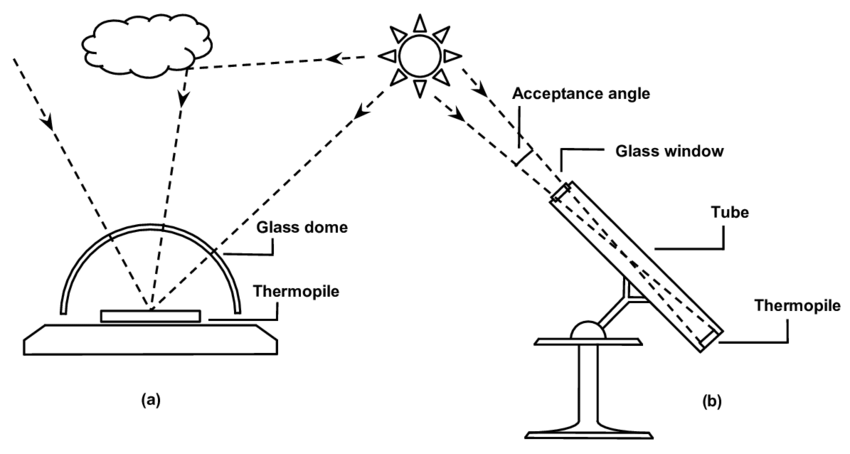
\includegraphics{images/Illustration-of-a-pyranometer-a-and-a-pyrheliometer.png}

\begin{columns}[T]
\begin{column}{0.5\textwidth}
\textbf{GHI} or \emph{Global}

Global Horizontal Irradiance
\end{column}

\begin{column}{0.5\textwidth}
\textbf{DNI} or \emph{Direct}

Direct Normal Irradiance
\end{column}
\end{columns}

~

\marginnote{\begin{footnotesize}

Image: https://www.sevensensor.com/what-is-pyranometer

\end{footnotesize}}
\end{block}
\end{frame}

\begin{frame}[fragile]
\begin{block}{Typical spectral responce}
\protect\hypertarget{typical-spectral-responce}{}
\includegraphics{images/energies-14-02766-g003.webp}

~ ~ ~ ~ ~ ~

\marginnote{\begin{footnotesize}

~ Mubarak R, Schilke H, Seckmeyer G. Improving the Irradiance Data
Measured by Silicon-Based Sensors. Energies. 2021; 14(10):2766.
doi:10.3390/en14102766

\end{footnotesize}}
\end{block}

\begin{block}{Have you seen those on the roof?}
\protect\hypertarget{have-you-seen-those-on-the-roof}{}
\begin{columns}[T]
\begin{column}{0.5\textwidth}
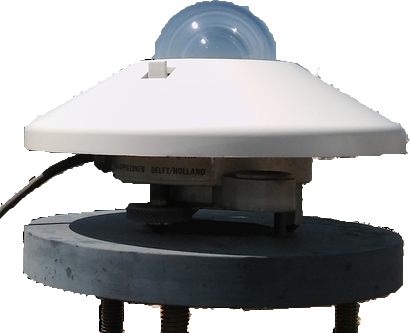
\includegraphics{images/cm21.png}
\end{column}

\begin{column}{0.5\textwidth}
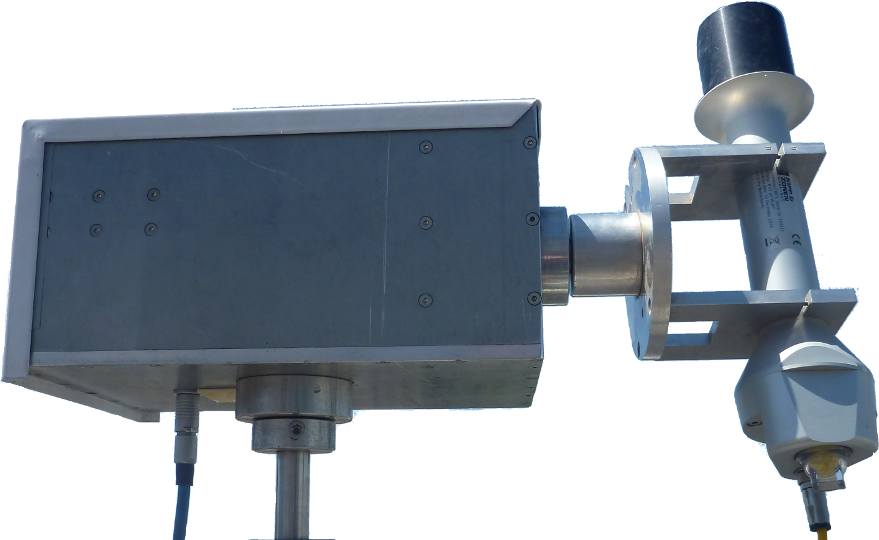
\includegraphics{images/P1110595e2.png}
\end{column}
\end{columns}

\begin{columns}[T]
\begin{column}{0.5\textwidth}
\textbf{Pyranometer CM-21.}

Global Horizontal Irradiance
\end{column}

\begin{column}{0.5\textwidth}
\textbf{Pyrheliometer CHP-1}

Direct Normal Irradiance
\end{column}
\end{columns}
\end{block}

\begin{block}{How we processed data here}
\protect\hypertarget{how-we-processed-data-here}{}
In brief\ldots{}

\begin{columns}[T]
\begin{column}{0.5\textwidth}
\begin{itemize}
\tightlist
\item
  Raw data

  \begin{itemize}
  \tightlist
  \item
    Inspect / Clean
  \item
    Convert to Watt/m\textsuperscript{2}
  \item
    Quality control
  \end{itemize}
\end{itemize}
\end{column}

\begin{column}{0.5\textwidth}
\begin{itemize}
\tightlist
\item
  Data grouping

  \begin{itemize}
  \tightlist
  \item
    All Sky conditions
  \item
    Clear Sky conditions
  \end{itemize}
\item
  Aggregation

  \begin{itemize}
  \tightlist
  \item
    Daily
  \item
    Monthly
  \end{itemize}
\end{itemize}
\end{column}
\end{columns}

~ ~

\marginnote{\begin{footnotesize}

~ If you use CM-21 data, ask for an update, or wait for refresh on
\texttt{sirena}

\end{footnotesize}}
\end{block}
\end{frame}

\begin{frame}{Results}
\protect\hypertarget{results}{}
\begin{block}{All sky conditions}
\protect\hypertarget{all-sky-conditions}{}
\begin{figure}

\begin{minipage}[t]{0.50\linewidth}

{\centering 

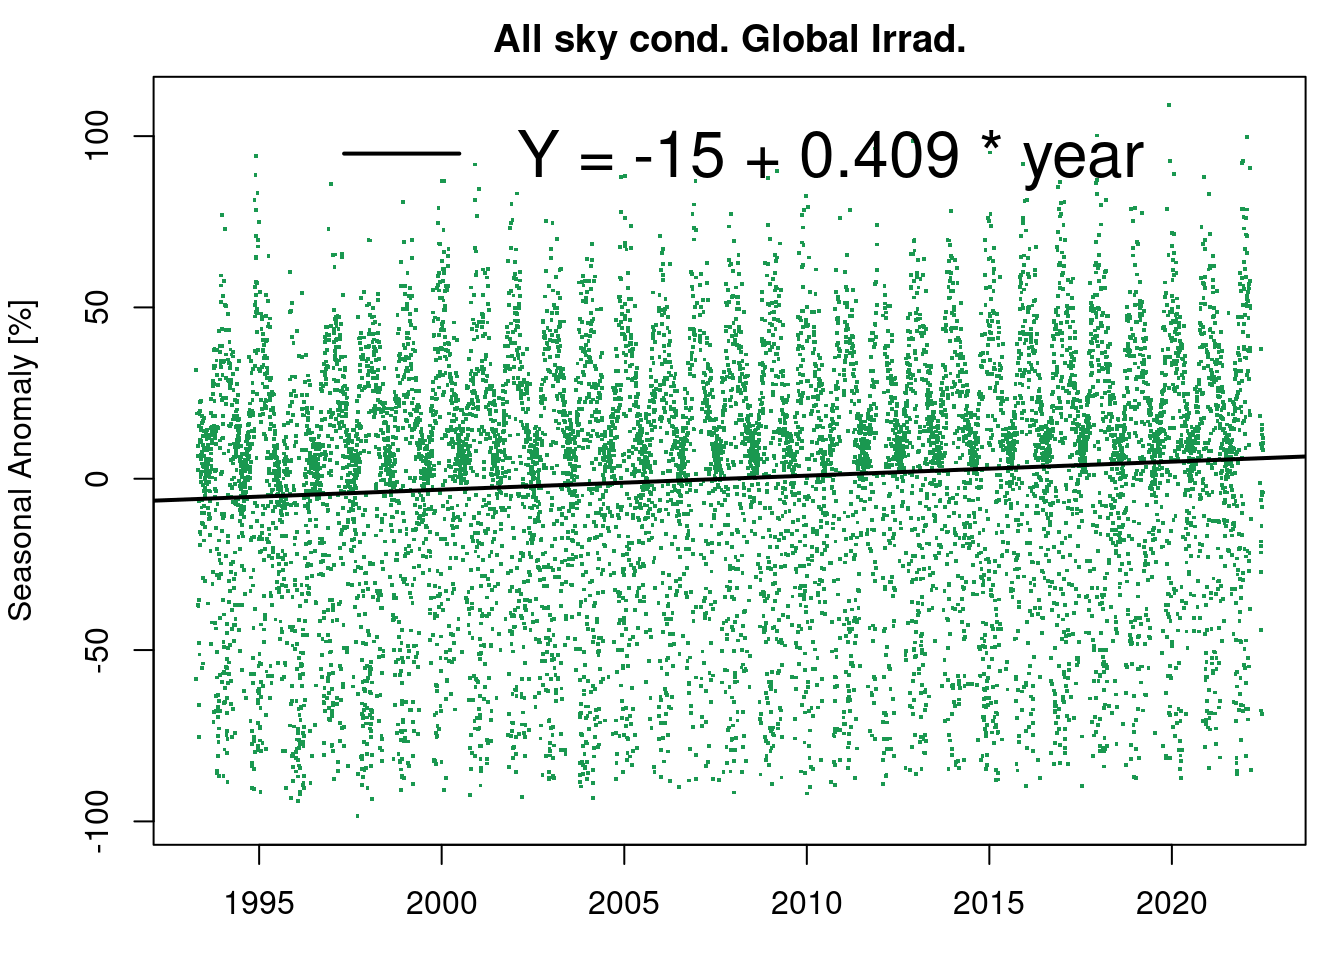
\includegraphics[width=4.48in,height=\textheight]{images/DHI_GHI_1_longterm_trends_files/figure-html/longtermtrendsALL-4.png}

}

\end{minipage}%
%
\begin{minipage}[t]{0.50\linewidth}

{\centering 

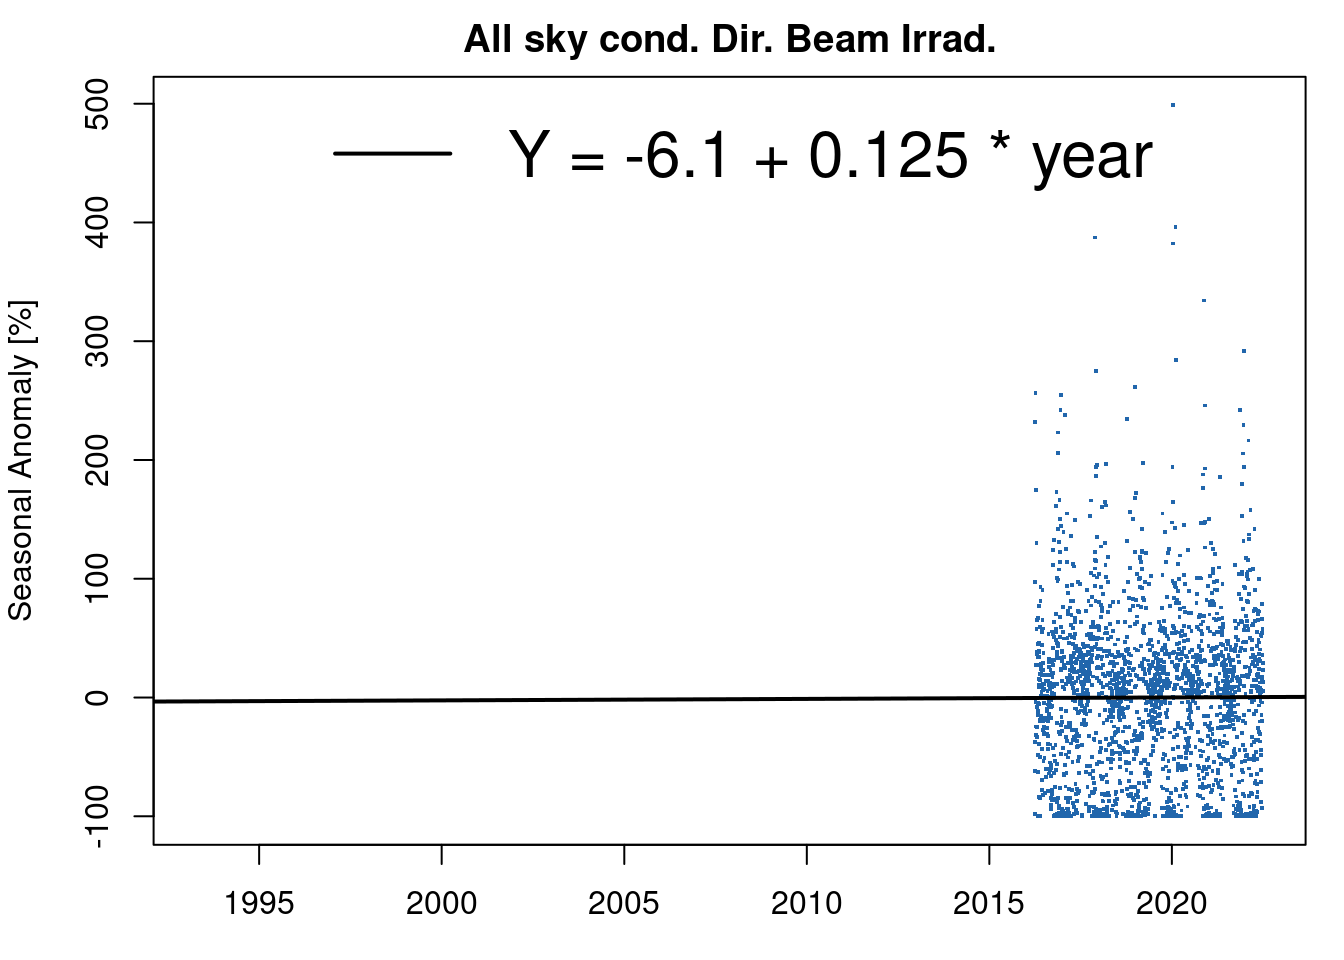
\includegraphics[width=4.48in,height=\textheight]{images/DHI_GHI_1_longterm_trends_files/figure-html/longtermtrendsALL-3.png}

}

\end{minipage}%

\end{figure}
\end{block}

\begin{block}{Clear sky conditions}
\protect\hypertarget{clear-sky-conditions}{}
\begin{figure}

\begin{minipage}[t]{0.50\linewidth}

{\centering 

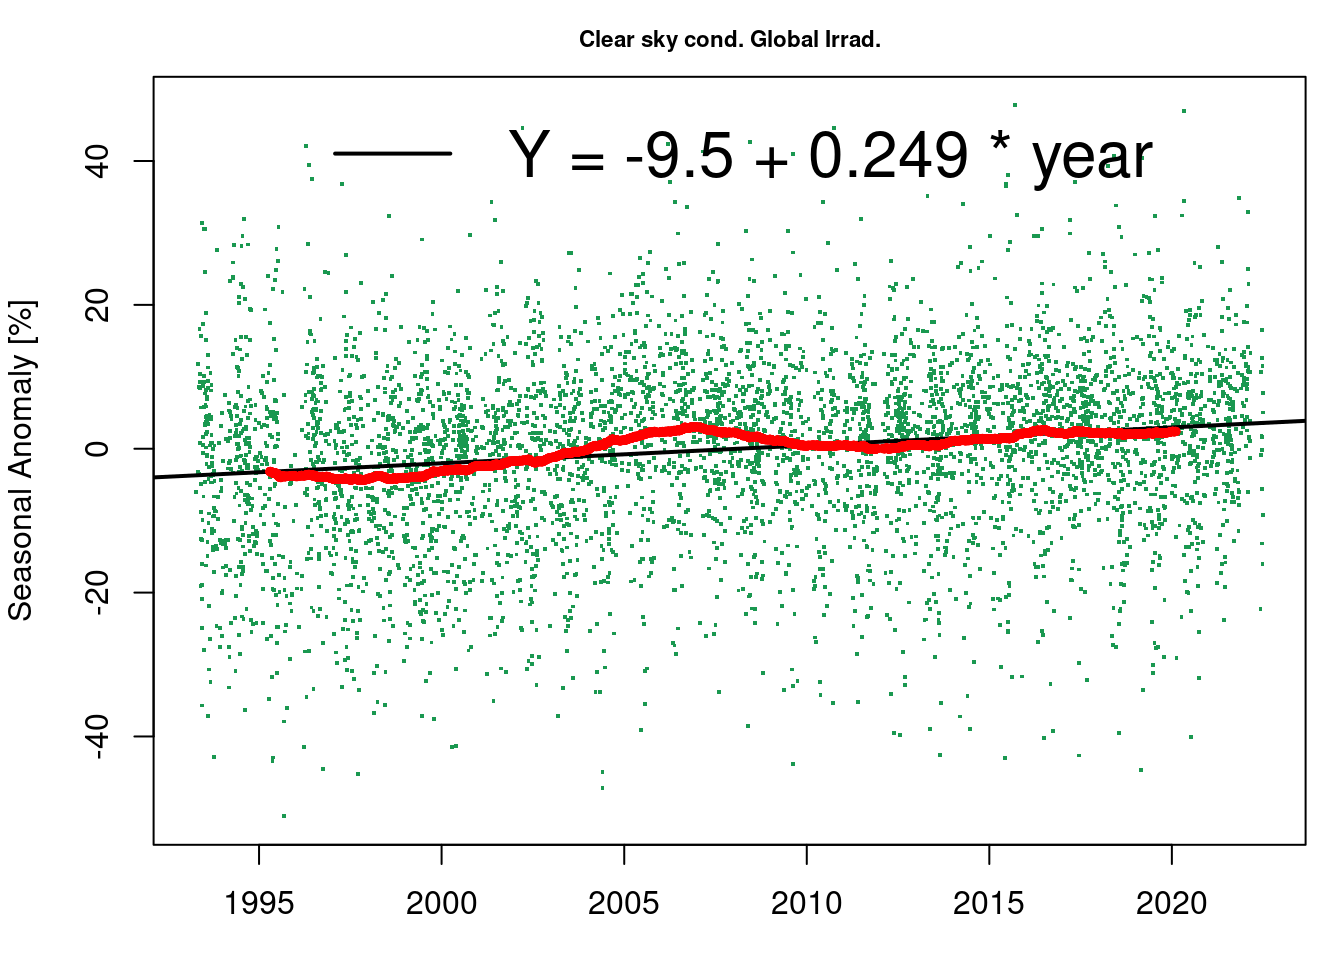
\includegraphics[width=4.48in,height=\textheight]{images/DHI_GHI_1_longterm_trends_files/figure-html/longtermtrendsCS-4.png}

}

\end{minipage}%
%
\begin{minipage}[t]{0.50\linewidth}

{\centering 

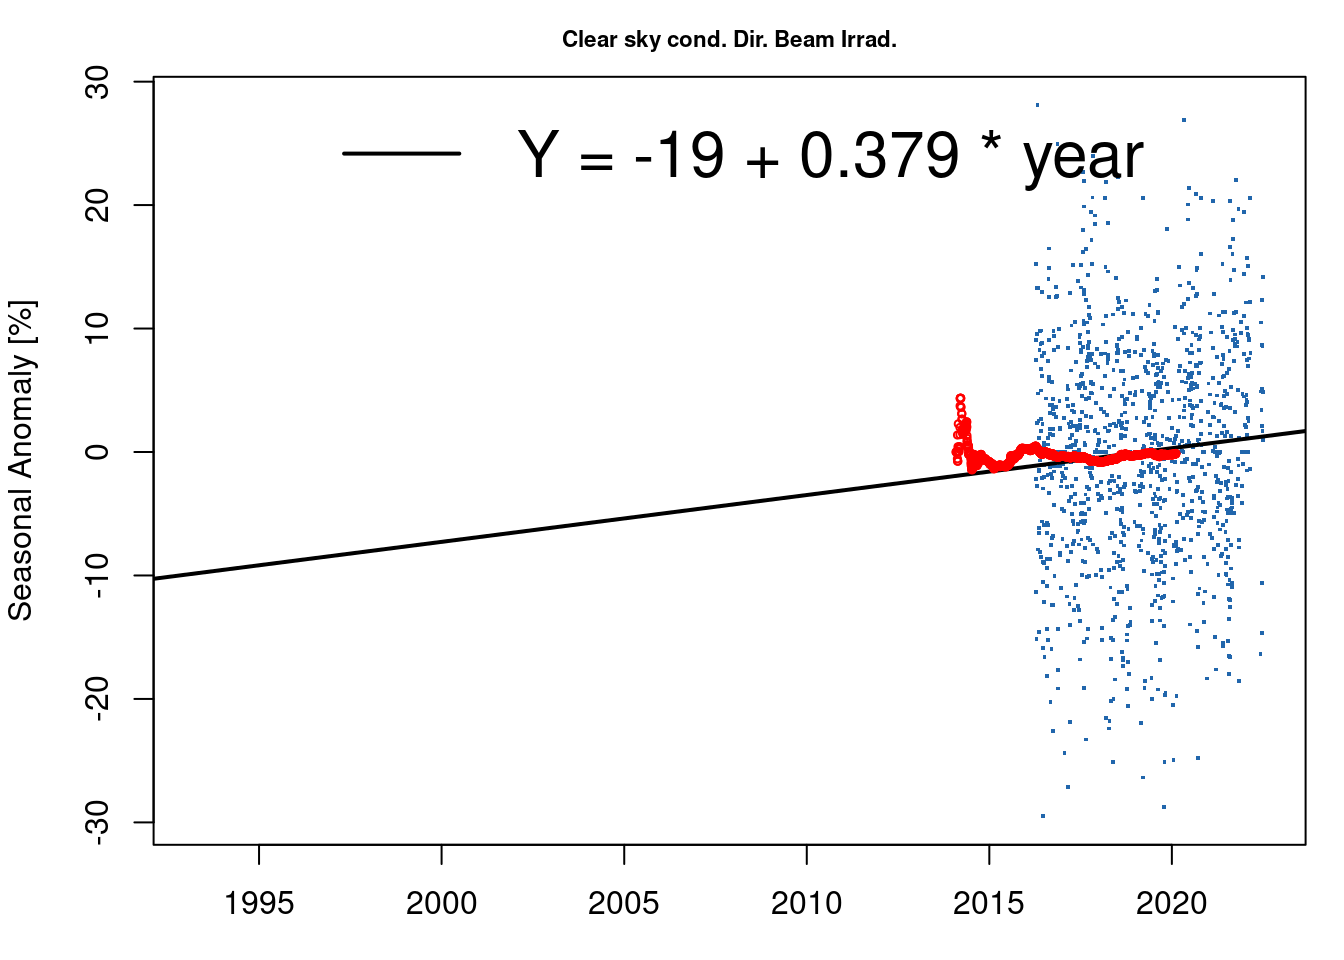
\includegraphics[width=4.48in,height=\textheight]{images/DHI_GHI_1_longterm_trends_files/figure-html/longtermtrendsCS-3.png}

}

\end{minipage}%

\end{figure}
\end{block}

\begin{block}{All data trends}
\protect\hypertarget{all-data-trends}{}
\begin{tabular}{>{}l|>{}l|>{}r|r}
\hline
Sky Cond. & Variable & Change per year [\%] & Statistical signif. [\%]\\
\hline
\textcolor{0}{ALL} & \textcolor{0}{Direct Beam} & \textcolor{0}{\sout{12.5}} & 12.0\\
\hline
\textcolor{blue}{ALL} & \textcolor{blue}{Global} & \textcolor{blue}{\textbf{40.9}} & 100.0\\
\hline
\textcolor{blue}{CLEAR} & \textcolor{blue}{Direct Beam} & \textcolor{blue}{\textbf{37.9}} & 98.6\\
\hline
\textcolor{blue}{CLEAR} & \textcolor{blue}{Global} & \textcolor{blue}{\textbf{24.9}} & 100.0\\
\hline
\end{tabular}

\note{Ignoring low statistical significance the rest shows an increasing
trend for most of the cases}
\end{block}

\begin{block}{Are the trends consistent ?}
\protect\hypertarget{are-the-trends-consistent}{}
Cumulative sum of deseasonalized monthly means\ldots{}

\begin{figure}

\begin{minipage}[t]{0.50\linewidth}

{\centering 

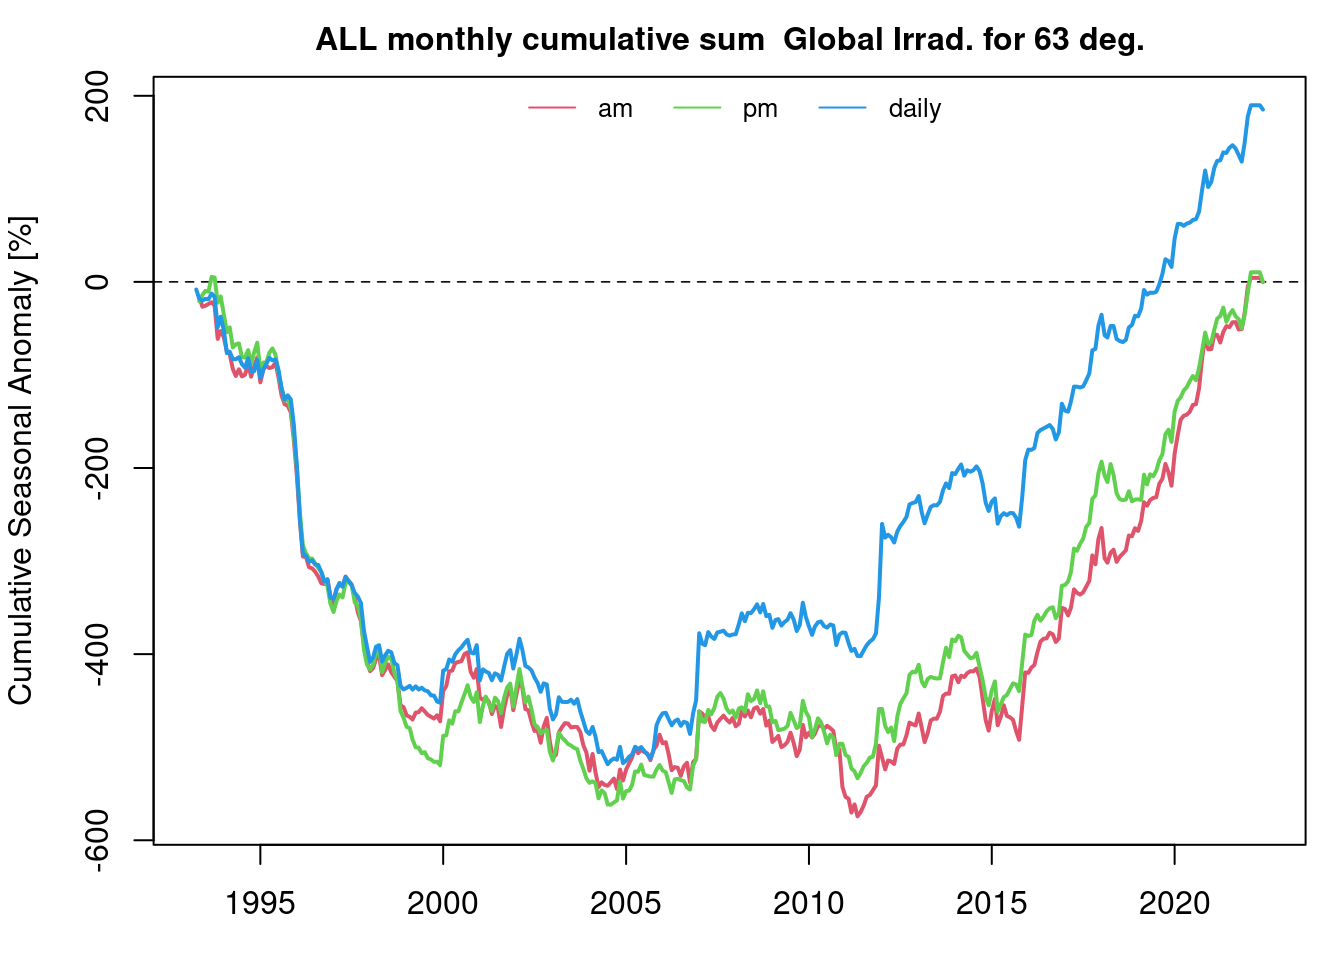
\includegraphics[width=4.48in,height=\textheight]{images/DHI_GHI_3_trends_consistency_files/figure-html/cumulativesums-1.png}

}

\end{minipage}%
%
\begin{minipage}[t]{0.50\linewidth}

{\centering 

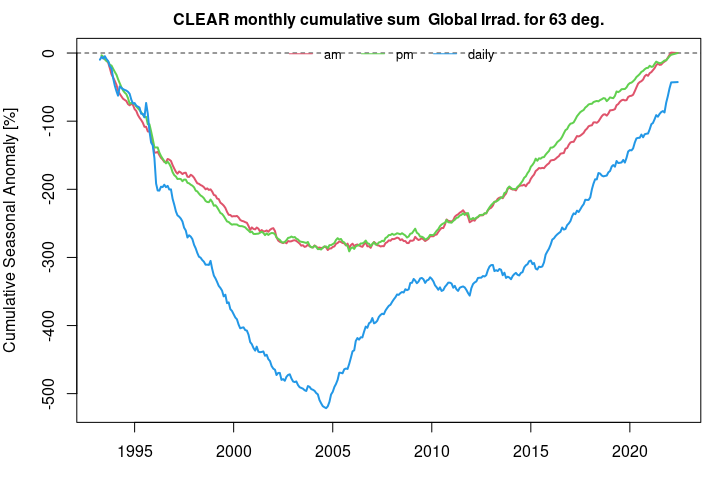
\includegraphics[width=4.48in,height=\textheight]{images/DHI_GHI_3_trends_consistency_files/figure-html/cumulativesums-4.png}

}

\end{minipage}%

\end{figure}

~

\marginnote{\begin{footnotesize}

Monthly means of deseasonlized daily means. Cumulative sum of monthly
means. For a specific SZA (63).

\end{footnotesize}}
\end{block}

\begin{block}{SZA dependency by Season \textasciitilde{} ALL SKY}
\protect\hypertarget{sza-dependency-by-season-all-sky}{}
\begin{figure}

\begin{minipage}[t]{0.50\linewidth}

{\centering 

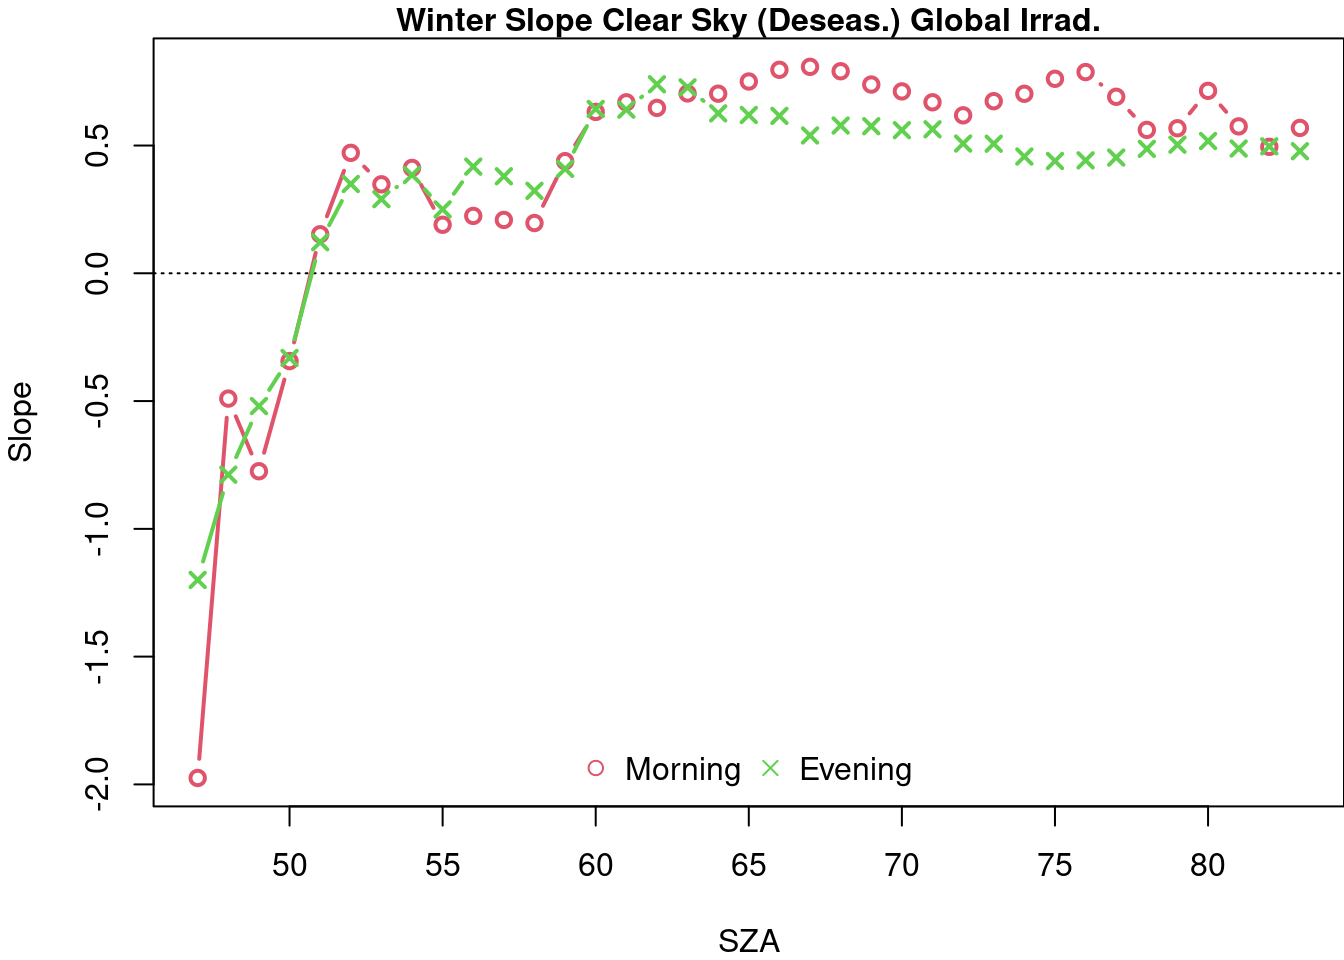
\includegraphics[width=4.48in,height=\textheight]{images/DHI_GHI_2_sza_trends_files/figure-html/szatrendsseas-6.png}

}

\end{minipage}%
%
\begin{minipage}[t]{0.50\linewidth}

{\centering 

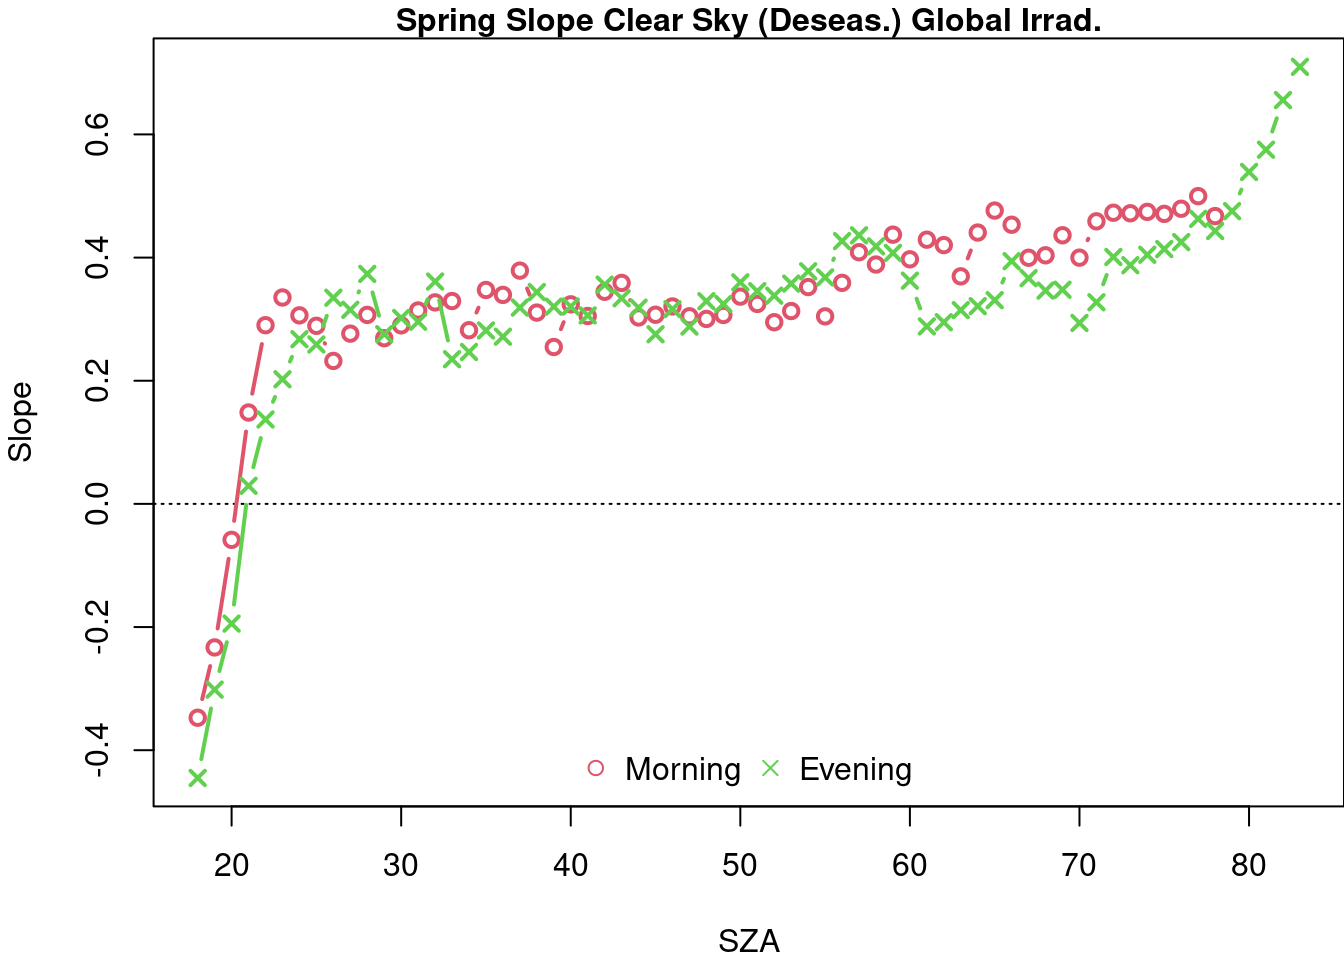
\includegraphics[width=4.48in,height=\textheight]{images/DHI_GHI_2_sza_trends_files/figure-html/szatrendsseas-36.png}

}

\end{minipage}%
\newline
\begin{minipage}[t]{0.50\linewidth}

{\centering 

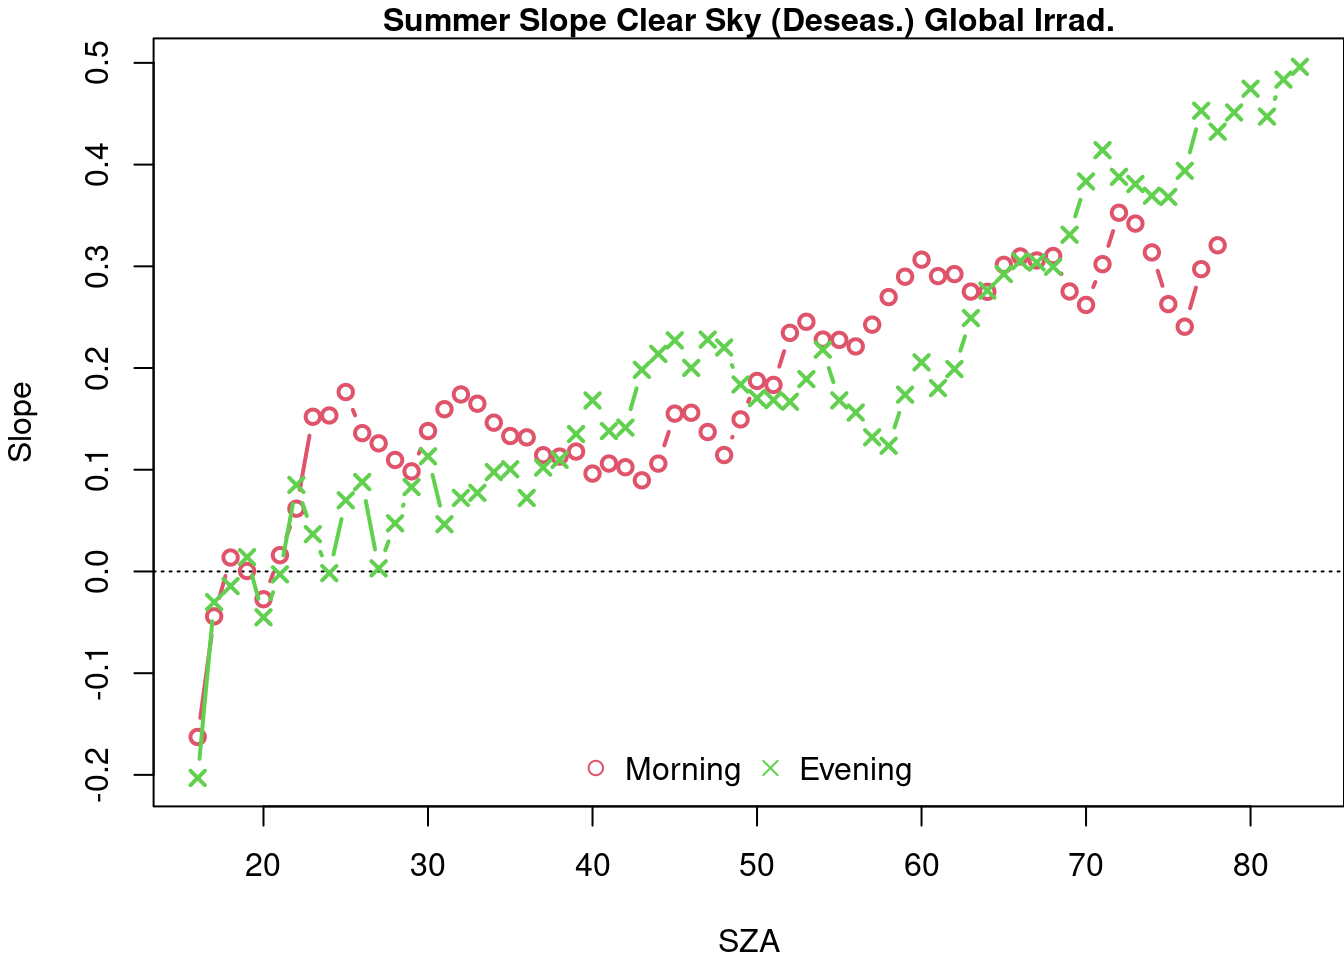
\includegraphics[width=4.48in,height=\textheight]{images/DHI_GHI_2_sza_trends_files/figure-html/szatrendsseas-66.png}

}

\end{minipage}%
%
\begin{minipage}[t]{0.50\linewidth}

{\centering 

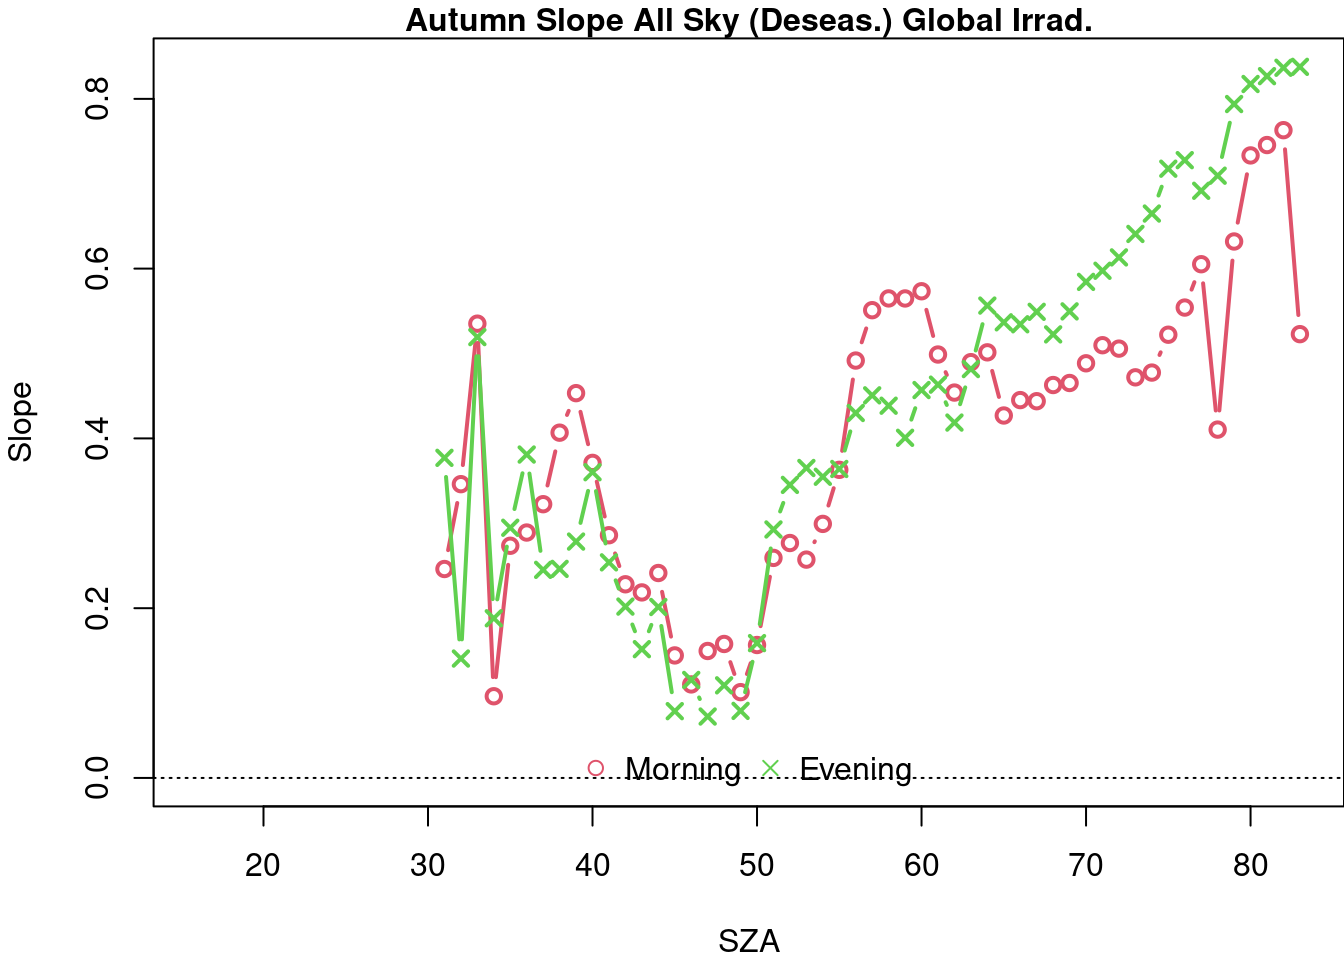
\includegraphics[width=4.48in,height=\textheight]{images/DHI_GHI_2_sza_trends_files/figure-html/szatrendsseas-96.png}

}

\end{minipage}%

\end{figure}
\end{block}

\begin{block}{SZA dependency by Season \textasciitilde{} CLEAR SKY}
\protect\hypertarget{sza-dependency-by-season-clear-sky}{}
\begin{figure}

\begin{minipage}[t]{0.50\linewidth}

{\centering 

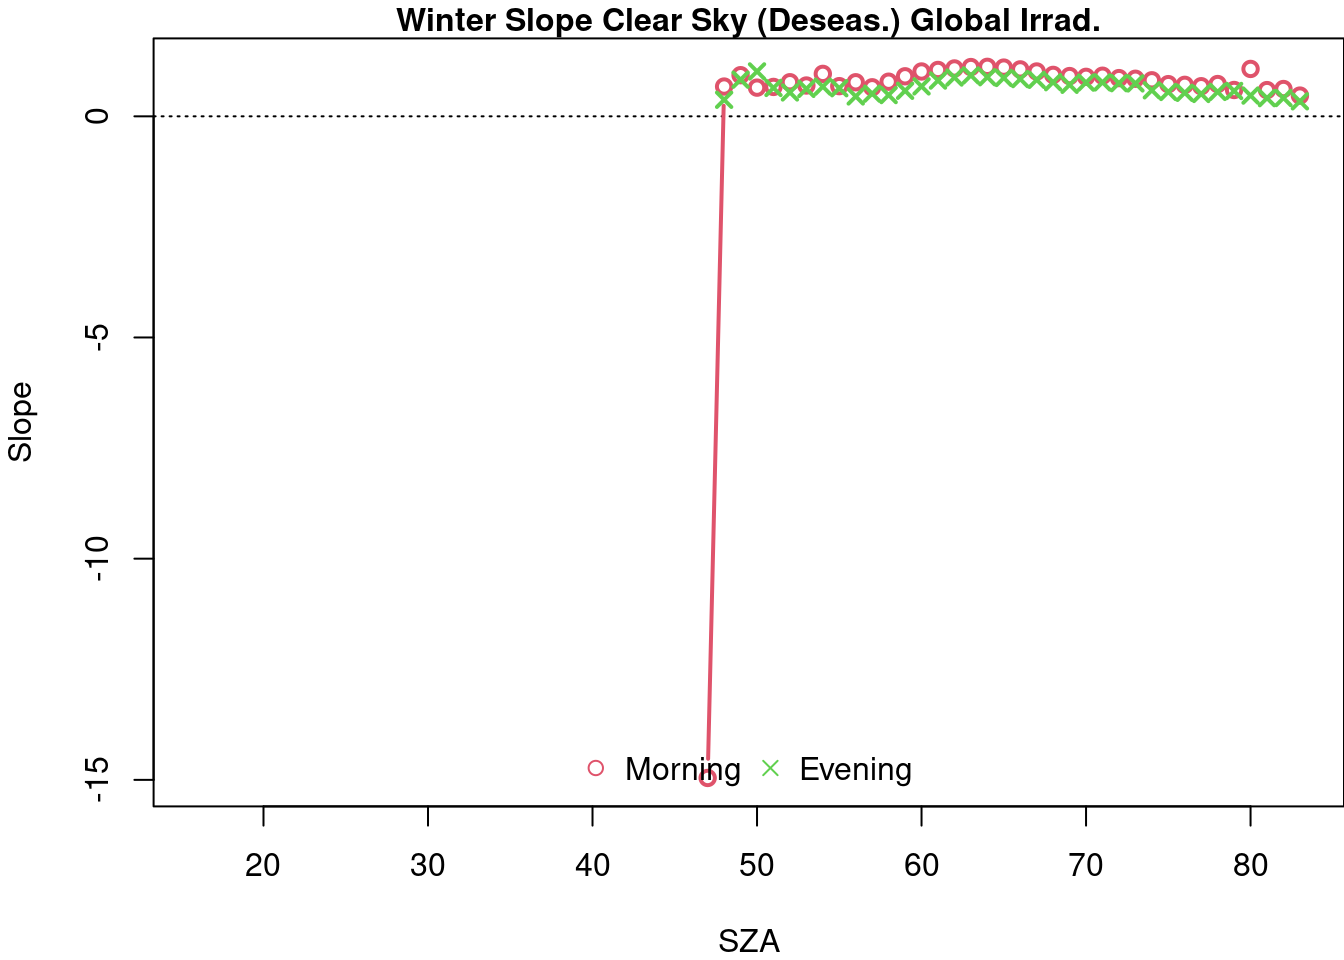
\includegraphics[width=4.48in,height=\textheight]{images/DHI_GHI_2_sza_trends_files/figure-html/szatrendsseas-21.png}

}

\end{minipage}%
%
\begin{minipage}[t]{0.50\linewidth}

{\centering 

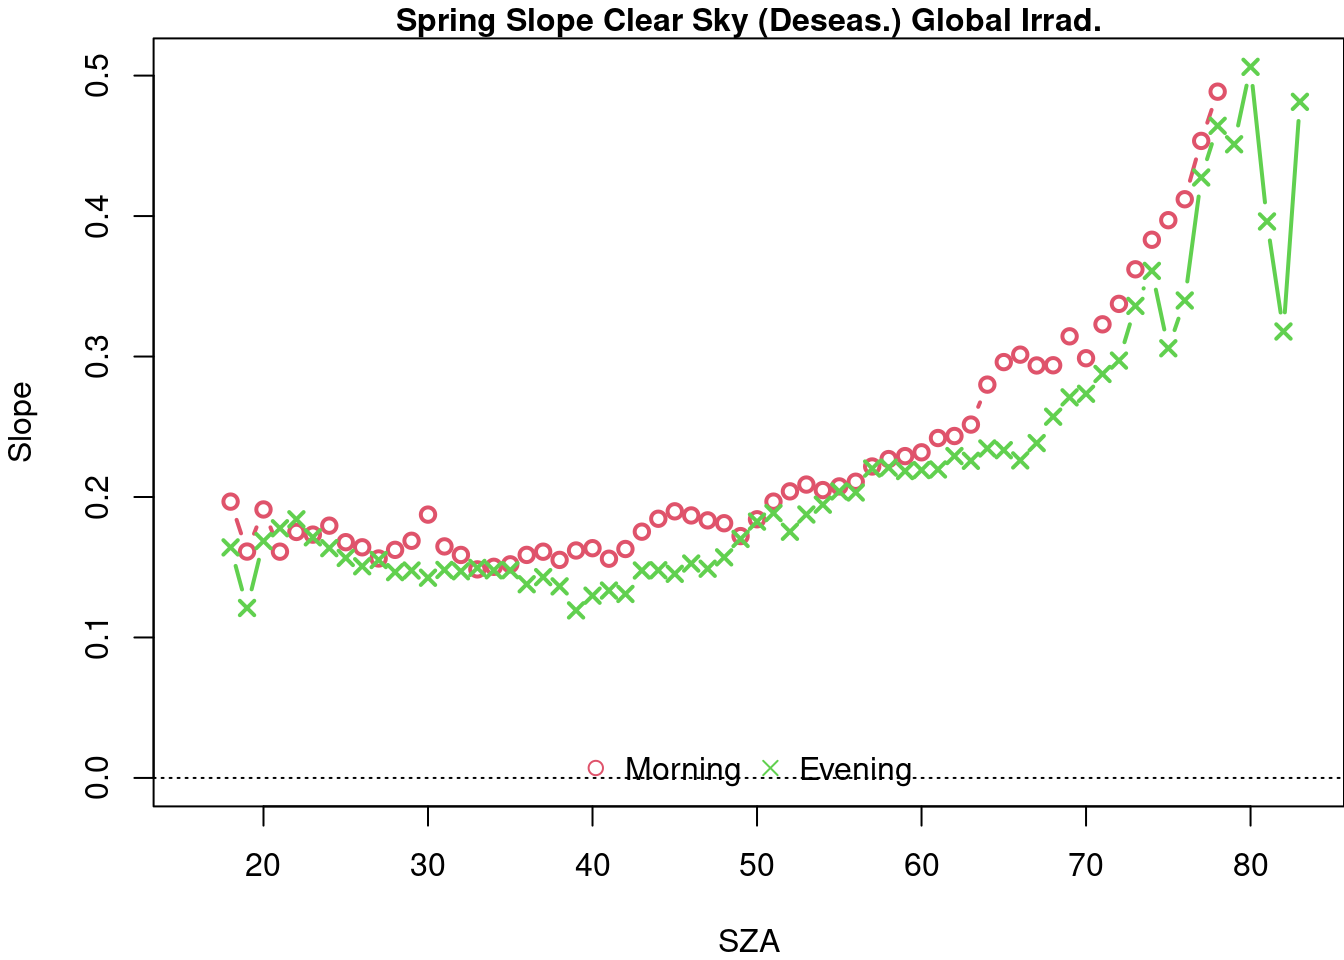
\includegraphics[width=4.48in,height=\textheight]{images/DHI_GHI_2_sza_trends_files/figure-html/szatrendsseas-51.png}

}

\end{minipage}%
\newline
\begin{minipage}[t]{0.50\linewidth}

{\centering 

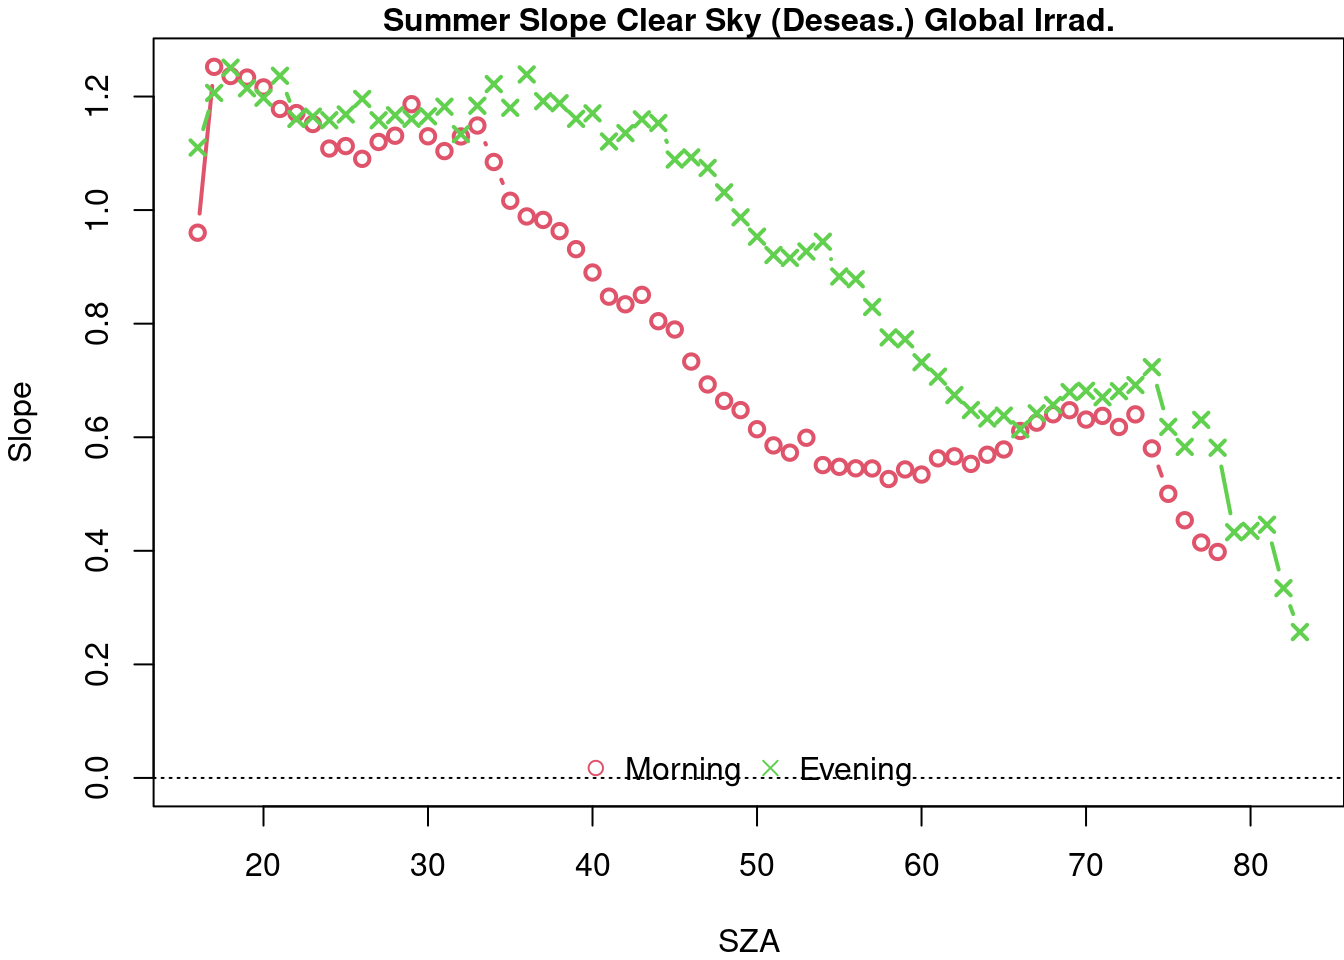
\includegraphics[width=4.48in,height=\textheight]{images/DHI_GHI_2_sza_trends_files/figure-html/szatrendsseas-81.png}

}

\end{minipage}%
%
\begin{minipage}[t]{0.50\linewidth}

{\centering 

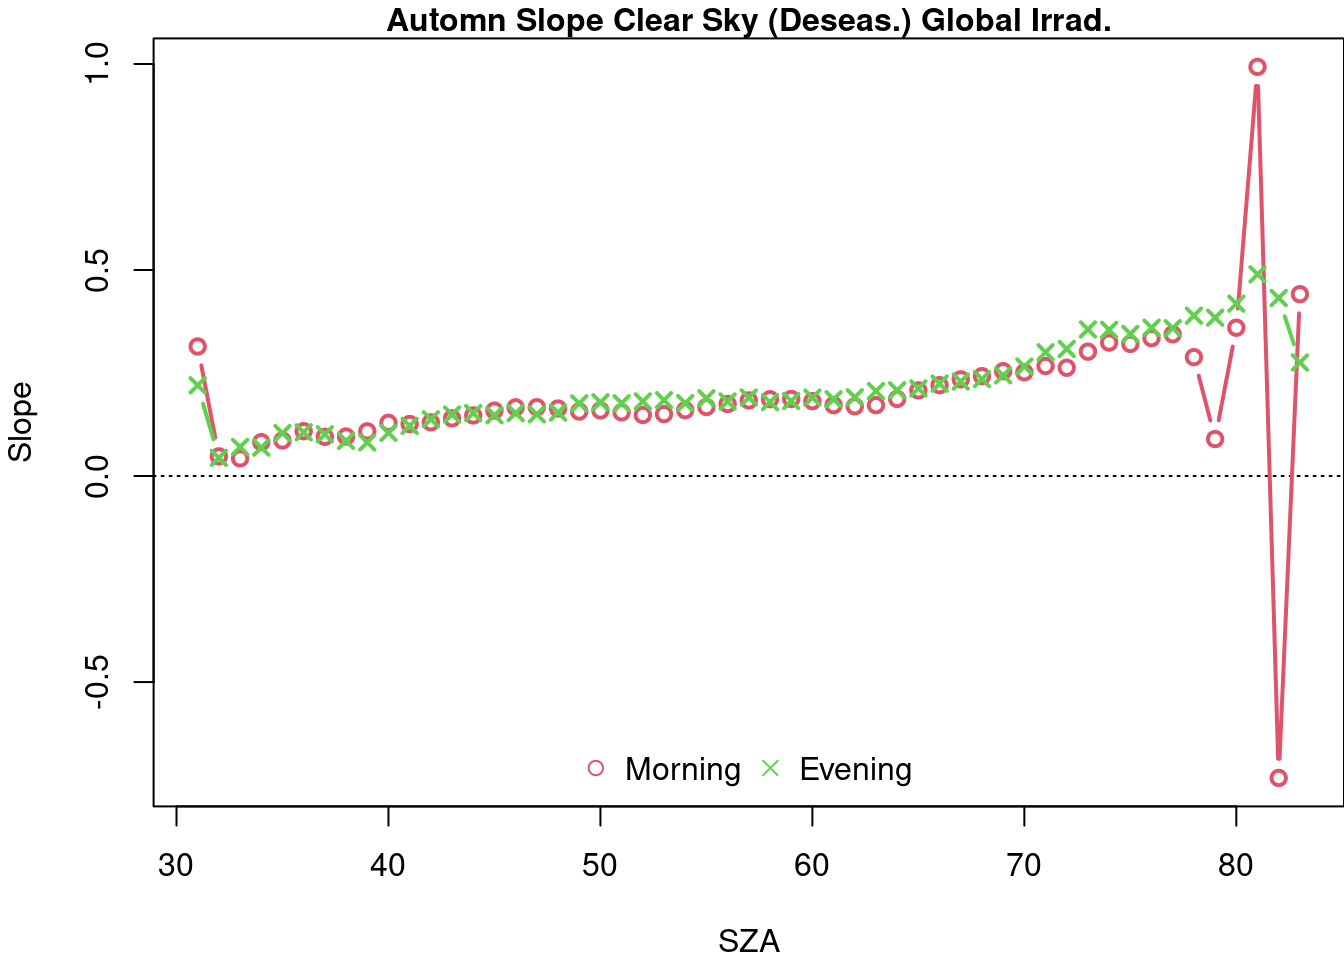
\includegraphics[width=4.48in,height=\textheight]{images/DHI_GHI_2_sza_trends_files/figure-html/szatrendsseas-111.png}

}

\end{minipage}%

\end{figure}
\end{block}

\begin{block}{Concluding}
\protect\hypertarget{concluding}{}
\begin{block}{We observed:}
\protect\hypertarget{we-observed}{}
\begin{itemize}
\tightlist
\item
  We observe an \textbf{increasing Global Shortwave Radiation}

  \begin{itemize}
  \tightlist
  \item
    Thessaloniki
  \item
    Brightening, last \textasciitilde30 years
  \item
    On Ground level
  \item
    Also in \textbf{Direct Beam Radiation} \footnote<.->{Short time
      series yet!}
  \end{itemize}
\item
  Similar results from other sources.
\end{itemize}

~ ~
\end{block}
\end{block}

\begin{block}{Concluding}
\protect\hypertarget{concluding-1}{}
\begin{block}{We care}
\protect\hypertarget{we-care}{}
\begin{itemize}
\tightlist
\item
  Depends on Anthropocentric activities

  \begin{itemize}
  \tightlist
  \item
    Aerosols \ldots{}
  \end{itemize}
\item
  Dimming on other time scales/regions
\item
  Effects Climate

  \begin{itemize}
  \tightlist
  \item
    Radiation balance
  \item
    Modeling
  \item
    Solar productivity
  \end{itemize}
\end{itemize}

~

\marginnote{\begin{footnotesize}

Key term: \textbf{Global Dimming and Brightening}

\end{footnotesize}}
\end{block}
\end{block}

\begin{block}{Concluding}
\protect\hypertarget{concluding-2}{}
\begin{block}{We want to}
\protect\hypertarget{we-want-to}{}
\begin{itemize}
\tightlist
\item
  Understand what drives the phenomenon in Thessaloniki

  \begin{itemize}
  \tightlist
  \item
    What dependencies can find with other factors/causes
  \end{itemize}
\item
  Is there any other locally useful information

  \begin{itemize}
  \tightlist
  \item
    Weather patterns
  \item
    Aerosol emission patterns
  \item
    \ldots{}
  \end{itemize}
\end{itemize}

~

\marginnote{\begin{footnotesize}

Keyword: Global Dimming and Brightening

\end{footnotesize}}
\end{block}
\end{block}
\end{frame}

\begin{frame}
~~~~Thank you ! ~~~~

~ ~

mail:~~\href{mailto:natsisthanasis@gmail.com}{\nolinkurl{natsisthanasis@gmail.com}}

The presentation will be available here (hopefully):
\url{https://github.com/thanasisn/presentations}
\end{frame}



\end{document}
